\documentclass{standalone}\usepackage[]{graphicx}\usepackage[]{color}
% maxwidth is the original width if it is less than linewidth
% otherwise use linewidth (to make sure the graphics do not exceed the margin)
\makeatletter
\def\maxwidth{ %
  \ifdim\Gin@nat@width>\linewidth
    \linewidth
  \else
    \Gin@nat@width
  \fi
}
\makeatother

\definecolor{fgcolor}{rgb}{0.345, 0.345, 0.345}
\newcommand{\hlnum}[1]{\textcolor[rgb]{0.686,0.059,0.569}{#1}}%
\newcommand{\hlstr}[1]{\textcolor[rgb]{0.192,0.494,0.8}{#1}}%
\newcommand{\hlcom}[1]{\textcolor[rgb]{0.678,0.584,0.686}{\textit{#1}}}%
\newcommand{\hlopt}[1]{\textcolor[rgb]{0,0,0}{#1}}%
\newcommand{\hlstd}[1]{\textcolor[rgb]{0.345,0.345,0.345}{#1}}%
\newcommand{\hlkwa}[1]{\textcolor[rgb]{0.161,0.373,0.58}{\textbf{#1}}}%
\newcommand{\hlkwb}[1]{\textcolor[rgb]{0.69,0.353,0.396}{#1}}%
\newcommand{\hlkwc}[1]{\textcolor[rgb]{0.333,0.667,0.333}{#1}}%
\newcommand{\hlkwd}[1]{\textcolor[rgb]{0.737,0.353,0.396}{\textbf{#1}}}%
\let\hlipl\hlkwb

\usepackage{framed}
\makeatletter
\newenvironment{kframe}{%
 \def\at@end@of@kframe{}%
 \ifinner\ifhmode%
  \def\at@end@of@kframe{\end{minipage}}%
  \begin{minipage}{\columnwidth}%
 \fi\fi%
 \def\FrameCommand##1{\hskip\@totalleftmargin \hskip-\fboxsep
 \colorbox{shadecolor}{##1}\hskip-\fboxsep
     % There is no \\@totalrightmargin, so:
     \hskip-\linewidth \hskip-\@totalleftmargin \hskip\columnwidth}%
 \MakeFramed {\advance\hsize-\width
   \@totalleftmargin\z@ \linewidth\hsize
   \@setminipage}}%
 {\par\unskip\endMakeFramed%
 \at@end@of@kframe}
\makeatother

\definecolor{shadecolor}{rgb}{.97, .97, .97}
\definecolor{messagecolor}{rgb}{0, 0, 0}
\definecolor{warningcolor}{rgb}{1, 0, 1}
\definecolor{errorcolor}{rgb}{1, 0, 0}
\newenvironment{knitrout}{}{} % an empty environment to be redefined in TeX

\usepackage{alltt}
%% recommended packages

%% more packages 
\usepackage{amsmath, tikz} % for table, equations, and flow chart figure (respectively)
\usetikzlibrary{fit, positioning, shapes} % for flow chart figure
\IfFileExists{upquote.sty}{\usepackage{upquote}}{}
\begin{document}

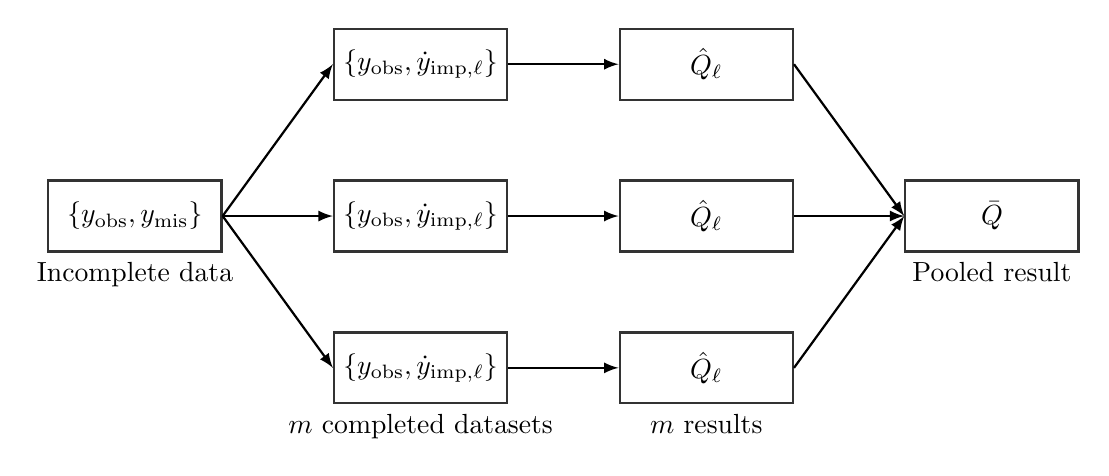
\begin{tikzpicture}
\tikzstyle{main}=[rectangle, minimum width = 22mm, minimum height = 9mm, thick, draw =black!80, node distance = 14mm]
\tikzstyle{connect}=[draw, -latex, thick, out=180,in=270, looseness=0]
\node[main, fill = white!100] (data) [label=below:Incomplete data] {$\{y_{\rm obs}, y_{\rm mis}\}$};
\node[main] (mids) [right=of data] { $\{y_{\rm obs}, \dot y_{\rm imp, \ell}\}$};
\node[main] (mids2) [above=10mm of mids] {$\{y_{\rm obs}, \dot y_{\rm imp, \ell}\}$ };
\node[main] (mids3) [below=10mm of mids,label=below: $m$ completed datasets] { $\{y_{\rm obs}, \dot y_{\rm imp, \ell}\}$};
\node[main] (mira) [right=of mids] {$\hat{Q}_\ell$};
\node[main] (mira2) [above=10mm of mira] { $\hat{Q}_\ell$ };
\node[main] (mira3) [below=10mm of mira,label=below: $m$ results] { $\hat{Q}_\ell$ };
\node[main, fill = white!100] (mipo) [right=of mira,label=below:Pooled result] {$\bar{Q}$ };
\path      
    (data.east) edge [connect] node [right] {} (mids.west)
(data.east) edge [connect] node [right] {} (mids2.west)
(data.east) edge [connect] node [right] {} (mids3.west)
      (mids.east) edge [connect] node [right] {} (mira.west)
      (mids2.east) edge [connect] node [right] {} (mira2.west)
      (mids3.east) edge [connect] node [right] {} (mira3.west)
		(mira.east) edge [connect] node [right] {} (mipo.west)
		(mira2.east) edge [connect] node [right] {} (mipo.west)
		(mira3.east) edge [connect] node [right] {} (mipo.west)
;
\end{tikzpicture}
%\caption{Scheme of the main steps in multiple imputation \citep[$m = 3$; adapted from][\S~1.4.1]{buur18}. {\footnotesize Missing data in dataset $Y$ is `imputed' (i.e., filled in) $m$ times. The imputed data is combined with the observed data ($Y_{obs}$) to create $m$ completed datasets. On each completed dataset, the analysis of scientific interest (or `substantive model') is performed. The quantity of scientific interest (e.g., a regression coefficient) is denoted with $Q$. Since $Q$ is estimated on each completed dataset, $m$ separate $\hat{Q}$-values are obtained. These $m$ values are combined into a single pooled estimate $\bar{Q}$. $\{y_{obs}, y_{mis}\}$ }} 


\end{document}
